\section{Assignment 15}

\subsection{Implement the parallel force/position control}

\begin{figure}[h]
\centering
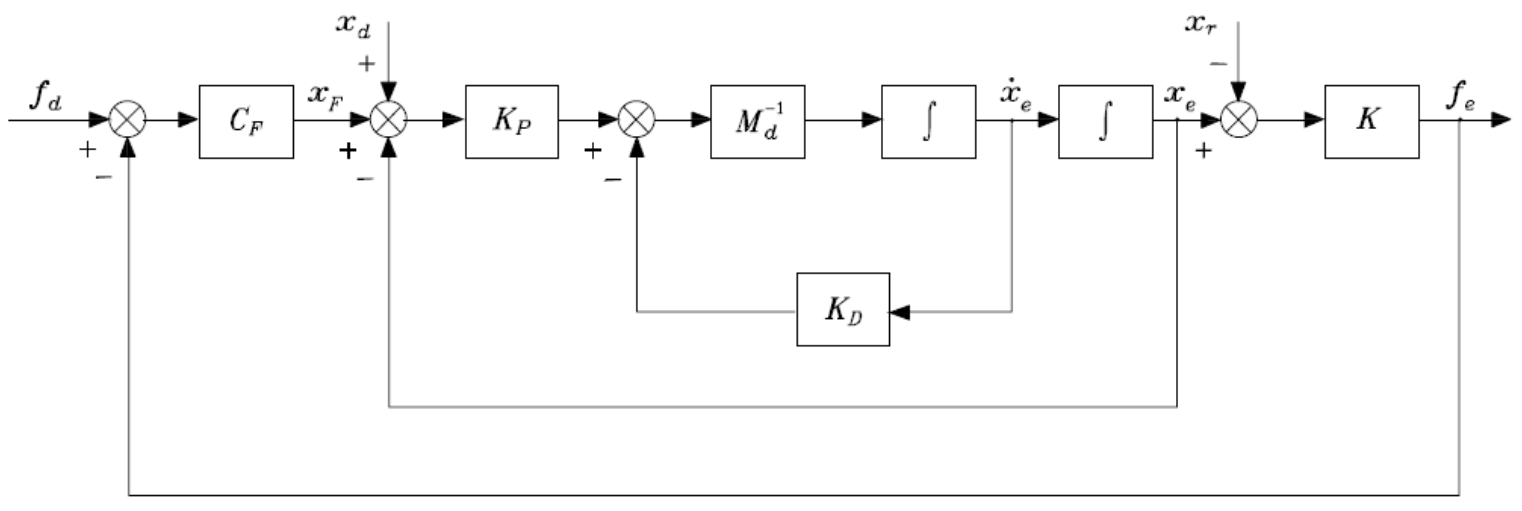
\includegraphics[keepaspectratio,width=0.8\textwidth]{parallel_arch}
\caption{Parallel force/position control architectures.}
\end{figure}

The architecture is essentially the same as the force control with inner position loop. The main difference is that we actually introduce the desired end-effector pose $x_d$ into  the position loop.

The architecture is implemented in SIMULINK as follows:

\begin{figure}[h]
\centering
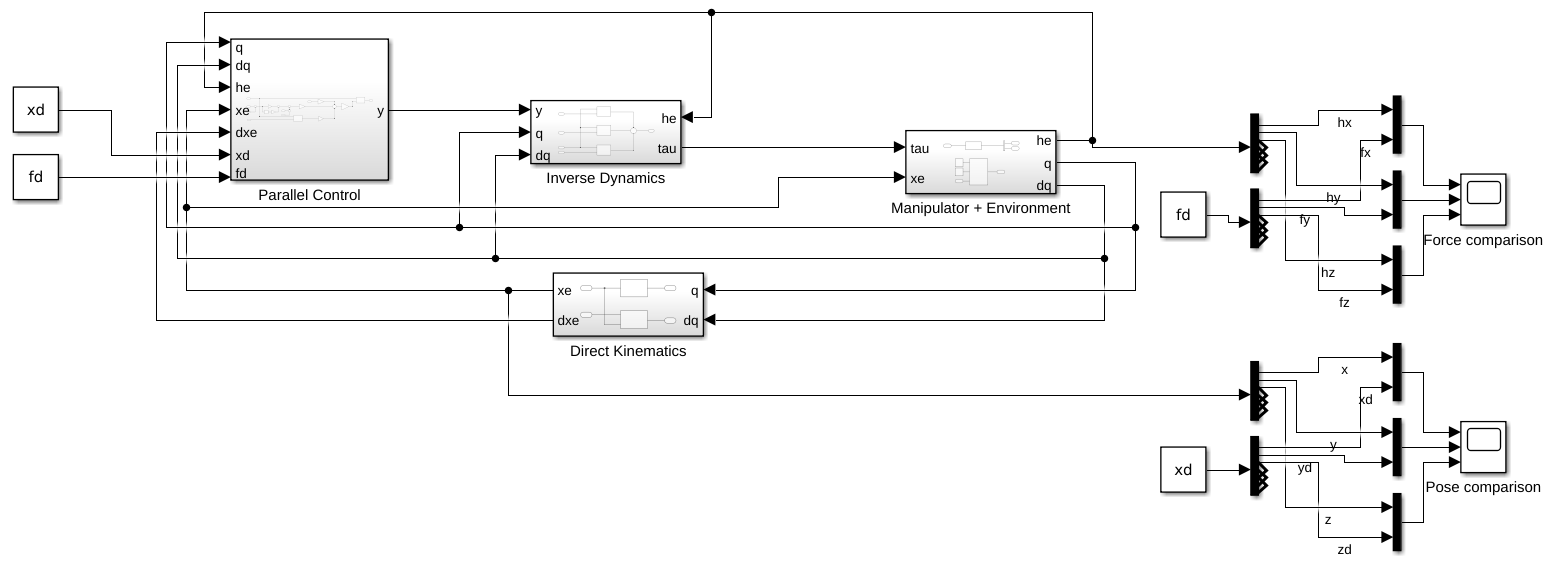
\includegraphics[keepaspectratio,width=0.8\textwidth]{parallel_sim}
\caption{Parallel force/position control SIMULINK model.}
\end{figure}

\newpage

The architecture was tested with $f_d = \begin{bmatrix}
0.5 & 0 & 0 & 0 & 0 & 0
\end{bmatrix}$, with an environment stiffness $K=\begin{bmatrix}
1 & 0 & 0 & 0 & 0 & 0
\end{bmatrix}$, PI gains for the force loop $K_I=15\mathbb I_6$ and $K_F=15\mathbb I_6$. The desired pose is $k(\begin{bmatrix}
-\pi/2 & -0.1 & -\pi/6
\end{bmatrix})$ while the environment is placed at  $k(\begin{bmatrix}
-\pi/2 & -0.2 & -\pi/6
\end{bmatrix})$.

\begin{figure}[h]
\centering
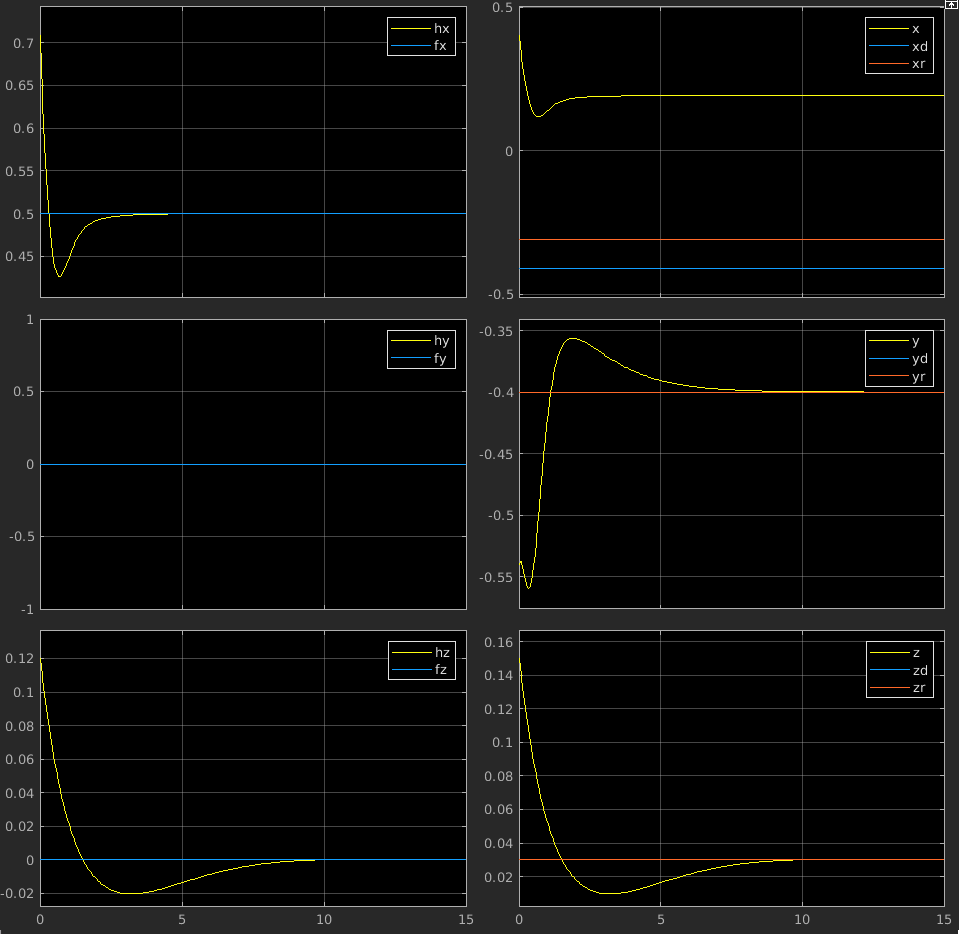
\includegraphics[keepaspectratio,width=0.8\textwidth]{parallel}
\caption{Parallel force/position control}
\end{figure}